% !TeX spellcheck = en_US
\documentclass[
	english,
	openany,
	draft = false,
	twoside = true,
	fleqn
]{scrbook}
\usepackage{learning-notes}

\author{Huu Duc Nguyen}
\authordegreefront{}
\authordegreeback{ M.Sc.}
\subject{AI}
\title{AI Notes}
\date{29 February 2022}

\begin{document}
\frontmatter
\TitlePage
\tableofcontents

\mainmatter
% !TeX spellcheck = en_GB

\chapter*{Abbreviations}
\addcontentsline{toc}{chapter}{Abbreviations}

\begin{acronym}[LONGEST]
	\acro{AI}{Artificial Intelligence}
	\acro{ML}{Machine Learning}
	\acro{DL}{Deep Learning}
	\acro{CS}{Computer Science}
	\acro{CV}{Computer Vision}
	\acro{RL}{Reinforcement Learning}
	\acro{NLP}{Natural Language Processing}
	
	\acro{prob}[prob.]{probability}
	\acro{param}[params.]{parameters}
	\acro{algor}[algor.]{algorithms}
	\acro{info}[info.]{information}
	\acro{aka}[a.k.a.]{also known as}
	\acro{no}[no.]{number of}
	\acro{func}[func.]{function}
	\acro{vs}[vs.]{versus}
	\acro{iid}[i.i.d.]{independent \& identically distributed}
	\acro{LSI}{linear shift invariant}
	
	\acro{pdf}[PDF]{Probability Density Function}
	\acro{MLE}{Maximum Likelihood Estimation}
	\acro{MAP}{Maximum A Posteriori}

	\acro{MoG}{Mixture of Gaussians}
	
	% Gradient descent
	\acro{nag}[NAG]{Nestorov Accelerated Gradient}
	\acro{rmsprop}[RMSprop]{Root mean squared prop}
	\acro{adam}[Adam]{Adaptive moment estimation}
	
	\acro{SVD}{Singular Value Decomposition}
	\acro{PCA}{Principal Component Analysis}
	\acro{LDA}{Linear Discriminant Analysis}
	\acro{kl}[K-L]{Kullback–Leibler}
	
	% Neural-network-related term
	\acro{relu}[ReLU]{Rectified Linear Unit}
\end{acronym}
% !TeX spellcheck = en_US
\chapter{Introduction}

\ac{AI} is the study field that leverages the ability of machines to mimic the problem-solving skill of human. In other words, \ac{AI} pushing machines to think, act like people, in a rational way. It lies in the core of countless novel applications in real life, self-driving cars, virtual assistant, face recognition, \etc. \ac{ML} is a sub-field of \ac{CS} and \ac{AI}, that “gives computers the ability to learn without being explicitly programmed” (\href{https://en.wikipedia.org/wiki/Machine_learning}{Wikipedia}). As a great amount of collected data and powerful computational hardware arise, \ac{DL} is then a subset of \ac{ML} (\figref{fig:relation-ai-ml-dl}). Advanced applications which relate to \ac{NLP}, \ac{CV}, robotic learning, \etc, are with in this \ac{DL} subset.
\begin{figure}[hbt!]
	\centering
	\includegraphics[width=1\textwidth]{nvidia-ai-ml-dl.jpg}
	\caption{The relation between \ac{AI}, \ac{ML} and \ac{DL} (\href{https://developer.nvidia.com/deep-learning}{src}).}
	\label{fig:relation-ai-ml-dl}
\end{figure}

It's important to understand that there are more to \ac{AI} and \ac{ML} than just neural networks. In the end, to create a meaningful and working neural network, one should have strong background in the basics of \ac{ML} as well.

These notes are my way of keeping record of what I have learn in the field. The structure of the notes is as follows:
\begin{itemize}
	\item \charef{cha:overview-ml} introduces common ideas in \ac{ML}.
	\item \charef{cha:probabilities} presents the mathematics background on probabilities, matrix.
	\item \todo{chapter 3} explain basic concepts, the branching of different classes in \ac{ML}. Later chapters presents each smaller branches.
\end{itemize}

\todo{The structure of the notes}
% !TeX spellcheck = en_US
\chapter{Overview of Machine Learning}

A machine learning algorithm is an algorithm that has the ability to \textit{learn} from the data. A computer program is said to \textbf{learn}, if its performance at tasks in $T$, measured by $P$, improves with experience $E$ (in which the experience is equivalent to the data). \cite{goodfellow2016deep}

\section{Task $T$}
A \textit{task} is usually described by how the \ac{ML} model process a single \textit{data point}. This section presents some common \ac{ML} tasks. \cite{vu2018mlcb}

\subsection{Classification}
The task is to specify a label for the given data point. The labels are usually members of a list.

\Eg, in the problem of digit classification, the data point is images of hand-written numbers. The data set comes with their labels as well. The task is then, given a unseen image, the model would be able to tell which number is in that image. In this problem, there are 10 possible labels, \ie, $0, 1, \dots, 9$.

\subsection{Regression}

\section{Experience $E$}
\section{Performance $P$}


% !TeX spellcheck = en_US
\chapter{Probabilities}
\label{cha:probabilities}

\section{Definitions}
\label{sec:prob-defs}

\subsection{Basic Definitions}
\begin{itemize}
	\item If $x$ is discrete: $\underset{x}{\sum} p(x) = 1$ with $\forall$ $0 \leq p(x) \leq 1$
	\item If $x$ is continuous: $\displaystyle \int p(x) \,dx = 1 \Rightarrow \exists$ a \textbf{\ac{pdf}}\\
	$p(x)$ can take any positive value, as long as \(\displaystyle \int p(x) \,dx = 1\)\\
	\todo{Add image}\\
	\note: theoretically $p(x) = 0, \forall x$
	\item Common types
	\begin{align*}
		& \text{Joint probability:} 		&& p(x_i, y_i) 	&& \left(= p(X=x_i, Y=y_i)\right) \\
		& \text{Marginal probability:} 		&& p(x_i) 		&& \left(= p(X=x_i)\right) \\
		& \text{Conditional probability:} 	&& p(y_i | x_i) && \left(= p(Y=y_i|X=x_i)\right)
	\end{align*}	
	\item Sum rule: $\displaystyle \sum$ joint \ac{prob} = marginal \ac{prob}\\
	$\Rightarrow$ Marginalization	
	\begin{itemize}
		\item discrete variable: $\displaystyle p(x)=\underset{y}{\sum} p(x, y)$
		\item continuous variable: $\displaystyle p(x) = \int p(x,y) dy$
	\end{itemize}
	\item Product rule: Product of marginal \ac{prob} and conditional \ac{prob} = joint \ac{prob}
\end{itemize}

\subsection{Independence and Variability}
\begin{itemize}
	\item Independence. \Eg: $x, y$ are independent, then
	\[\begin{cases}
		p(x|y) = p(x)\\
		p(y|x) = p(y)
	\end{cases}
	\iff p(x,y) = p(x).p(y)\]
	
	\item Variability
	\begin{itemize}
		\item variance:\\ $var \left[f\right] = \expectation{\left(f(x)-\expectation{f(x)}\right)^2} = \expectation{f(x)^2} - \expectation{f(x)}^2$
		\item covariance:\\ $cov \left[x, y\right] = \mathbb{E}_{x,y}\left[xy\right] - \expectation{x}.\expectation{y} = \mathbb{E}_{x,y}\left[xy^T\right] - \expectation{x}.\expectation{y^T}$
		\item covariance matrix
	\end{itemize}
\end{itemize}

\subsection{Bayes Rule}
\label{subsec:bayes-rule}
\begin{align*}
	& p(x_i|y_i).p(y_i) = p(y_i|x_i).p(x_i) = p(x_i, y_i) \\
	\Rightarrow\; &p(y_i|x_i) = \frac{p(x_i|y_i).p(y_i)}{p(x_i)} = \frac{p(x_i|y_i).p(y_i)}{\underset{y}{\sum} p(x_i|y_i).p(y_i)}
\end{align*}
$\Rightarrow$ the \hlb{Bayes equation}:\\~\\
\hlre{posterior = \frac{likelihood \times prior}{normalization~factor}}

\subsection{Expectation}
\label{subsec:expectation}
\begin{align*}
	& \text{For variable $x$:} && \expectation{x} = \underset{x}{\sum}x.p(x) && \left( = \int x.p(x)dx \right)\\
	& \text{For function $f(.)$:} && \expectation{f(x)} = \underset{x}{\sum}f(x).p(x) && \left( = \int f(x).p(x)dx \right)
\end{align*}

\section{Types of Probability Distributions}
Reference source: \href{https://machinelearningcoban.com/2017/07/09/prob/}{machinelearningcoban.com}.
\subsection{Bernoulli Distribution}
Bernoulli Distribution is a distribution to describe binary discrete variables. It's the case that the variable can only take value in 2 classes $x \in \{0,1\}$. \Eg, the probability of throwing a coin. The Bernoulli distribution is defined with parameter $\lambda \in[0,1]$:
\begin{equation}
	p(x) = \text{Bern}_x[\lambda] = \begin{cases}
		p(x=1) = \lambda\\
		p(x=0) = 1-\lambda
	\end{cases}
\end{equation}
In short form, the above equation can be combined into one:
\begin{equation}
	p(x) = \lambda^x(1-\lambda)^{(1-x)} \Rightarrow
	\begin{cases}
		p(0) = \lambda^0 (1-\lambda)^1 = 1-\lambda \\
		p(1) = \lambda^1 (1-\lambda)^0 = \lambda \\
	\end{cases}
\end{equation}

\subsection{Categorical Distribution}
\label{subsec:categorical-distribution}
\textit{Categorical Distribution} is the generalization of \textit{Bernoulli Distribution}, in case there are $K$ classes for the discrete variable $x \in \{ 1, 2, \dots, K\}$. Accordingly, there will be $K$ parameters to describe this \ac{pdf}: $\lambda = [\lambda_1, \lambda_2, \dots, \lambda_K]$, with $\lambda_k \geq 0$ and $\sum \lambda_k = 1$. Each $\lambda_k$ represents the probability to take the output $k$: $p(x = k) = \lambda_k$. In short: $p(x) = \text{Cat}_x [\lambda]$.

Another common way to represent the output is the one-hot vector, $\mathbf{x} \in \{\mathbf{e}_1, \mathbf{e}_2, \dots, \mathbf{e}_K\}$ with $\mathbf{e}_k$ is the $k$-unit vector, which has all 0-element, except the $k$-element equal to 1. \Eg, given 3 classes: $\textbf{e}_1 = [1, 0, 0]^T, \textbf{e}_2 = [0, 1, 0]^T, \textbf{e}_3 = [0, 0, 1]^T$. We will then have:
\begin{equation}
	p(\mathbf{x} = \mathbf{e}_k) = \prod_{j=1}^K \lambda_j^{x_j} = \lambda_k
\end{equation}
because for $\textbf{x}=\textbf{e}_k$, only $x_k=1$, while $x_j = 0, \forall j\neq k$.

\subsection{Univariate Normal Distribution}
Univariate Normal Distribution is also known as the Gaussian distribution. For single dimension data (in 1D): $x \in (-\infty, \infty)$, the mean $\mu \in \mathbb{R}$, and the variance $\sigma^2$ with $\sigma \in \mathbb{R}$.
\begin{equation}
	p(x) = \text{Norm}_x\left[\mu, \sigma^2\right] = \mathcal{N}(\mu, \sigma^2) = \frac{1}{\sqrt{2\pi\sigma^2}}.\text{exp}\left(-\frac{(x-\mu)^2}{2\sigma^2}\right)
\end{equation}
\note
\begin{itemize}
	\item \hlr{Marginals \ac{prob} of Gaussian are again Gaussian.}
	\item When estimating the \ac{param} of a Gaussian, beware the underestimation problem.
	\begin{align*}
		\expectation{\mu_{ML}} &= \mu \\
		\expectation{\sigma^2_{ML}} &= \left(\frac{N-1}{N}\right)\sigma^2 \\
		\Rightarrow \overset{\sim}{\sigma}^2 &= \left(\frac{N}{N-1}\right)\sigma^2_{ML} = \frac{1}{N-1} \sum_{n=1}^{N} (x_n-\hat{\mu})^2
	\end{align*}
\end{itemize}
\begin{figure}[hbt!]
	\centering
	\includegraphics[width=0.7\textwidth]{gaussian-pdf.png}
	\caption{Bivariate Gaussian distribution (\href{https://stats.stackexchange.com/questions/102632/plot-two-dimensional-gaussian-density-function-in-matlab}{src}).}
	\label{fig:relation-ai-ml-dl}
\end{figure}

\subsection{Multivariate Normal Distribution}
\textit{Multivariate Normal Distribution} is the extension of \textit{Univariate Normal Distribution} to multi-dimensional data: $\textbf{x}, \boldsymbol{\mu} \in \mathbb{R}^D, \sigma^2 \Rightarrow \Sigma \in \mathbb{S}^D_{++}$ ($\mathbb{S}^D_{++}$ is the set of positive definite symmetric matrix)
\begin{equation}
	p(x) = \text{Norm}_x [\boldsymbol{\mu}, \Sigma] = \mathcal{N}(\boldsymbol{\mu}, \Sigma) = \frac{1}{2\pi^{D/2}| \Sigma|^{\frac{1}{2}}} . \text{exp} \left( -\frac{1}{2} {(\textbf{x} - \boldsymbol{\mu})^T \Sigma^{-1} (\textbf{x} - \boldsymbol{\mu})} \right)
\end{equation}

\subsection{Beta Distribution}
This distribution describes the parameter for another distributions. \Eg, Dirichlet \ac{pdf} describes Categorical Distribution (\subsecref{subsec:categorical-distribution})

\section{Parameter Estimation}
Many of \ac{ML} problems are boiled down to finding \textit{statistical models}. Those models could predict the \ac{prob} for the classification problem, \ac{prob} of events that will happen, \etc. It all end up with finding the suitable set of \ac{param} for these \textit{statistical models}.
\subsection{Maximum Likelihood Estimation}
\ac{MLE} finds the parameters that maximize the \ac{prob} of the existing data.
\begin{align}
	& &&\theta = \underset{\theta}{\text{argmax}}\:p(x_1, x_2, \dots, x_N | \theta) \\
	&\text{Assuming independent variables:} &&\theta = \underset{\theta}{\text{argmax}} \prod^N_{n=1} p(x_n | \theta) \\
	&\text{Maximum log-likelihood:} &&\theta = \underset{\theta}{\text{argmax}} \sum^N_{n=1} \left[\text{log}\:p(x_n | \theta) \right]\\
	&\text{Minimum negative log-likelihood:} && \theta = \underset{\theta}{\text{argmin}} \sum^N_{n=1} \left[-\text{log}\:p(x_n | \theta)\right]
\end{align}

\subsection{Maximum A Posteriori}
Sometimes, we have prior knowledge of the \ac{pdf}. \Eg, we know that the \ac{prob} of getting head when flipping a coin is around 50\%. \ac{MAP} takes advantage of the prior knowledge $p(\theta)$ on the parameters $\theta$ by applying Bayes rule (\subsecref{subsec:bayes-rule})
\begin{equation}
	\theta = \underset{\theta}{\text{argmax}} \prod^N_{n=1} p(x_n | \theta)p(\theta)
\end{equation}
\hlr{\ac{MLE} suffers when there is not enough data} $\Rightarrow$ \hlr{use \ac{MAP}}

\section{Naive Bayes Classifier}
Naive implies having the independence assumption on the variables.
\begin{align*}
	c 	&= \underset{c \in \mathbb{C}}{\text{argmax}}\:p(c|x)\\
		&= \underset{c \in \mathbb{C}}{\text{argmax}}\:p(x|c)\,p(c)
\end{align*}

If $x$ is:
\begin{itemize}
	\item continuous variable $\Rightarrow$ Gaussian Naive Bayes
	\item feature vector $\Rightarrow$ Multinomial Naive Bayes
	\item binary vector $\Rightarrow$ Bernoulli Naive Bayes
\end{itemize}

Minimize the expected loss: $\displaystyle \expectation{L} = \sum_{k}\sum_{j}\int_{R_j}L_{kj}\,p(x, C_k)\,dx$ by choosing region $R_j$ such that $\displaystyle \expectation{L} = \sum_kL_{kj}\,p(C_k| x)$

\section{Views on the Decision Problem}
\subsection{\hlr{Generative Methods}}
First determine the class-conditional densities and separately infer the prior class \ac{prob} $\Rightarrow$ Bayes theorem $\Rightarrow$ class membership
\[p(x|C_k)\,p(C_k) \Rightarrow y_k(x)\]
\Eg, Mixture of Gaussians

\subsection{\hlr{Discriminative Methods}}
First solve the inference problem of determined the posterior class \ac{prob}

\section{Unknown Notes}
\Eg, 2 class $C_1, \; C_2$, 2 decisions $\alpha_1, \; \alpha_2$.

The loss: $L(\alpha_j | C_k) = L_{kj}$.

The expected loss is equal to the $Risk(R)$.
\begin{align*}
	\mathbb{E}_{\alpha_1}[L] = R(\alpha_1|x) = L_{11}\,p(C_1|x) + L_{21}\,p(C_2|x)\\
	\mathbb{E}_{\alpha_2}[L] = R(\alpha_2|x) = L_{12}\,p(C_1|x) + L_{22}\,p(C_2|x)\\
\end{align*}
Choose $\alpha_1$ if $R(\alpha_1|x) < R(\alpha_2|x)$

% !TeX spellcheck = en_US

\section{Probability Density Estimation}
\label{cha:pdf-estimation}

\subsection{Histogram}
This is \hlb{non-parametric} \ac{prob} density estimation. All other approaches are \hlb{parametric}. The \ac{prob} of a bin:
\begin{equation}
	p_i = \frac{n_i}{N.\Delta_i}
\end{equation}

in which $n_i$ is the number of data points in that bin, $N$ is the total number of data point, $\Delta_i$ is the width of the bin, often $\Delta_i=\Delta$.

\hlb{Notes}:
\begin{itemize}
	\item $\Delta$ serves as the \hlr{smoothing factor}
	\item With $D$ as the dimensions of the data points. The number of bins grow exponentially with $\mathcal{O}(k^D)$
\end{itemize}
\begin{figure}[hbt!]
	\centering
	\includegraphics[width=0.4\textwidth]{histogram.png}
	\caption{Example of a histogram, $\Delta = 1$ (\href{https://en.wikipedia.org/wiki/Histogram}{src}).}
\end{figure}

\subsection{Parametric Probability Density Estimation}
In the other hands, one could find the \ac{prob} from $\displaystyle p = \int_{\mathcal{R}}p(y)dy \approx p(x)V$ where the region $\mathcal{R}$ is sufficiently small.\\
$\displaystyle \Rightarrow p(x) \approx \frac{K}{N.V}$, where $K$ is the number of data points in the region, $V$ is the volume of the region.

\subsection{Kernel Methods}
The kernel methods fix $V$ and determine $K$. The volume $V$ is the space restricted within a parzen window $k(u)$ that satisfies $k(u) \geq 0$.
\begin{align}
	&\text{A hyper-space cube:} && k(u) = \begin{cases}
		1\;\; if \;\; |u_i| \leq \frac{1}{2}h, \;\; i = 1, 2, \dots, D \\
		0\;\; else
	\end{cases} \\
	&\text{The number of points inside:} &&K = \sum_{n=1}^{N} k(x-x_n) \\
	&\text{The region \textit{volume}:} &&V = \int k(u) du = h^D\\
	&\text{The probability:} && \Rightarrow p(x) \approx \frac{K}{N.V} = \frac{1}{N.h^D}\sum_{n=1}^{N}k(x-x_n)
\end{align}
The \hlb{symmetric Gaussian kernel is a better substitution} for the asymmetric parzen window.
\begin{align}
	&\text{A Gaussian kernel:} && k(u) = \frac{1}{\sqrt{2\pi h^2}}\:exp\left(\frac{-u^2}{2h^2}\right) \\
	&\text{The region \textit{volume}:} &&V = \int k(u) du = 1 \\
	&\text{The probability:} && \Rightarrow p(x) \approx \frac{1}{N} \sum_{n=1}^{N} \frac{1}{(2\pi)^{D/2}h}\:exp\left(\frac{-||x-x_n||^2}{2h^2}\right)
\end{align}
For Kernel methods, $h$ is the \hlb{smoothing factor}.

Generalization: $k(u) \geq 0$, $\displaystyle \int k(u)du = 1$.

\hlr{Size of the hypersphere is proportional to $h^2$.}

\subsection{K-Nearest Neighbor}
When you fix $K$ and determine $V$, it leads to K-Nearest Neighbor.

\todo{Add image}

\begin{equation}
	p(x) \approx \frac{K}{NV}
\end{equation}
Here, $K$ is the \hlb{smoothing factor}.

\hlr{\begin{itemize}
		\item Too much bias $\Rightarrow$ too smooth
		\item Too much variance $\Rightarrow$ \underline{NOT} smooth enough
	\end{itemize}
	$\Rightarrow$ combine parametric methods to a mixture model}

\hlr{Mixture distribution = multi parametric model}

\subsection{Mixture of Gaussians}
\ac{MoG}, as \hlr{Generative Model}, is defined from the \ac{prob} sum of elemental Gaussians: $\displaystyle p(x|\theta) = \sum_{j=1}^{M}p(x|\theta_j)p(j)$, where $p(x|\theta_j)$ is a \hlr{mixture component}, $p(j) = \pi_j$ is the \hlr{weight of the component}
\begin{align}
	p(x|\theta_j) &= \frac{1}{\sqrt{2\pi}\sigma_j}\:exp\left[\frac{-(x-\mu_j)^2}{2\sigma_j^2}\right],\;\;p(j)=\pi_j, \;\;\sum\pi_j=1 \\
	p(x|\theta_j) &= \frac{1}{(2\pi)^{\frac{D}{2}}|\Sigma_j|^{\frac{1}{2}}}\:exp\left[-\frac{1}{2}(x-\mu_j)^T\Sigma_j^{-1}(x-\mu_j)\right]
\end{align}

\subsection{K-Means Clustering}
There are 3 steps:
\begin{itemize}
	\item Pick $K$ centroids
	\item Assign sample to the centroid
	\item Adjust centroids
\end{itemize}

Step 2 and 3 are repeated until there is no change.

This leads to a local optimum, depends on initialization. It's sensitive to \hlb{outliers}, detects \hlb{spherical clusters only}.

\todo{Add images}

Application: \eg, image compression.

\subsection{EM Clustering}
It's short for Expectation-Maximization. Assuming $N$ data points and $K$ Gaussians.
\begin{itemize}
	\item \textbf{E-Step:} Fix the Gaussians, find $\gamma_j(x)$, which represent the \hlr{responsibility of component $j$ for $x$}.
	\begin{equation}
		\gamma_j(x_n) = \frac{\pi_j \mathcal{N}\left(x_n|\mu_j,\Sigma_j\right)}
		{\sum_{k=1}^{K}\pi_k \mathcal{N}\left(x_n|\mu_k,\Sigma_k\right)} \;\;\forall j=1, 2, \dots, K, \;\; n=1, 2, \dots, N
	\end{equation}	
	\item \textbf{M-Step:} Fix $\gamma_j(x)$, update the Gaussians.
	\begin{align}
		\hat{N}_j &= \sum_{n=1}^{N}\gamma_j(x_n) \\
		\hat{\mu}_j &= \frac{1}{\hat{N}_j} \sum_{n=1}^{N} \gamma_j(x_n)x_n \\
		\hat{\pi}_j &= \frac{\hat{N}_j}{N} \\
		\hat{\Sigma}_j &= \frac{1}{\hat{N}_j} \sum_{n=1}^{N} \gamma_j(x_n) \left(x_n - \hat{\mu}_j\right)\left(x_n - \hat{\mu}_j\right)^T
	\end{align}
\end{itemize}
\hlb{Notes}:
\begin{itemize}
	\item Regularization with $\Sigma + \sigma_{min}I$
	\item Initialization $\mu_j$ with K-Means
	\item Hard-assignment: each data point to 1 class $\Rightarrow$ K-Means
	\item Soft-assignment: each data point $\Rightarrow$ \ac{prob} to fall into many classes $\Rightarrow$ EM Clustering
\end{itemize}

EM \hlr{needs more iteration}, because there are \hlr{more \ac{param}}.
% !TeX spellcheck = en_US
\chapter{Basic ML Problems}

\section{Linear Regression}
This is the simplest regression problem in \ac{ML}.

\hlb{Problem statement:} Given data points $\textbf{x}_i \in \mathbb{R}^D$ and their labels $y_i \in \mathbb{R}$, find the \textit{line} that fits these data points. The line is represented via parameters $\textbf{w} = [w_0, w_1, \dots, w_n]^T$. For each data point $\textbf{x}$ and its label $y$.

\hlb{Approach:}
\begin{align*}
	\bar{\textbf{x}} &= [1, x_0, \dots, x_n] && \text{(x bar - extended variable)}\\
	y \approx \hat{y} &= \bar{\textbf{x}} . \textbf{w} && \text{(y hat - predicted label)}\\
	\Rightarrow \frac{1}{2}e^2 &= \frac{1}{2} \left(y - \bar{\textbf{x}}.\textbf{w}\right)^2 && \text{(the squared error between true and predicted labels)}
\end{align*}
\begin{align}
	\mathcal{L}(\textbf{w}) &= \frac{1}{2} \sum_{i=1}^{N} \left(y_i - \bar{\textbf{x}}_i.\textbf{w}\right) ^2 && \text{(the loss function for all points)} \\
	\mathcal{L}(\textbf{w}) &= \frac{1}{2N} \sum_{i=1}^{N} \left(y_i - \bar{\textbf{x}}_i.\textbf{w}\right) ^2 && \text{(the average loss)} \\
	\textbf{w}^* &= \underset{\textbf{w}}{\text{argmin}}\,\mathcal{L}(\textbf{w}) && \text{(the weights that minimize the loss function)} \\
	\mathcal{L}(\textbf{w}) &= \frac{1}{2} ||\textbf{y}-\overline{\textbf{X}}.\textbf{w}||^2_2 && \text{(using matrix form)}
\end{align}

with $\overline{\textbf{X}} = \begin{bmatrix}
	\bar{\textbf{x}}_1 \\
	\bar{\textbf{x}}_2 \\
	\vdots \\
	\bar{\textbf{x}}_n
\end{bmatrix}$
and $\textbf{y} = \begin{bmatrix}
	y_1 \\
	y_2 \\
	\vdots \\
	y_n	
\end{bmatrix}$

\hlb{Solution:}
\begin{align}
	&\frac{\partial\mathcal{L}(\textbf{w}^*)}{\partial\textbf{w}} = \overline{\textbf{X}}^T \left( \overline{\textbf{X}} \textbf{w}^* - \textbf{y} \right) = 0 \\
	\Leftrightarrow \; &\overline{\textbf{X}}^T\overline{\textbf{X}}\textbf{w}^* = \overline{\textbf{X}}^T \textbf{y} \\
	\Leftrightarrow \; &\textbf{w}^* = \left( \overline{\textbf{X}}^T \overline{\textbf{X}} \right)^\dagger \overline{\textbf{X}}^T \textbf{y}
\end{align}
in which, $A^\dagger$ (A dagger) is the pseudo inverse of a matrix, because $A$ might not be inverse-able. {\color{red} \boxed{A^\dagger = \left(A^TA\right)^{-1}A^T}}

\note
\begin{itemize}
	\item Sensitive to outliers $\Rightarrow$ pre-processing
	\item Multi-variable:
	\begin{align*}
		\mathcal{L}(\textbf{w}) &= \frac{1}{2N} ||\textbf{y}-\overline{\textbf{X}}.\textbf{w}||^2_2 \\
		\Rightarrow\; \nabla_\textbf{w}\mathcal{L}(\textbf{w}) &= \frac{1}{N} \overline{\textbf{X}}^T (\overline{\textbf{X}}\textbf{w}-\textbf{y})
	\end{align*}
\end{itemize}

\section{Linear Discriminant Functions}
\label{sec:linear-classification}
\hlb{Problem statement:} of general classification problem
\begin{itemize}
	\item Given: training set $\textbf{X} = \{\textbf{x}_1, \textbf{x}_2, \dots, \textbf{x}_N\}$ with target values (labels) $\textbf{T} = \{\textbf{t}_1, \textbf{t}_2, \dots, \textbf{t}_N\}$.
	\item Goal: take a new input $\textbf{x}$ and assign it to one of $K$ classes $C_k$\\
	$\Rightarrow$ Learn a discriminant function $y(x)$ to perform the classification
\end{itemize}
\hlb{Approach:}
\begin{itemize}
	\item 2-class problem: Binary target values: $t_n \in \{0, 1\}$\\
	\Eg of discriminant function: $y(x) > 0 \Rightarrow$ class $C_1$, else $C_2$
	\item K-class problem: 1-of-K coding scheme, \eg: $\textbf{t}_n = [0, 1, 0, 0, 0]^T$
	\item Extension to multiple classes: one-vs-all, one-vs-one classifiers
\end{itemize}

\subsection{Least-squares classification}
With above problem statement, consider $K$ classes described by linear models:
\begin{align*}
	y_k(\textbf{x}) &= \textbf{w}^T_k\textbf{x} + w_{k0} && k=1, \dots, K \\
	\Rightarrow \textbf{y}(\textbf{x}) &= \widetilde{\textbf{W}}^T\widetilde{\textbf{x}} && \text{(using vector notation)} \\
	\textbf{Y}(\widetilde{\textbf{X}}) &= \widetilde{\textbf{X}}\widetilde{\textbf{W}} && \text{(for the entire dataset)}
\end{align*}
In which output $\textbf{y}$ in 1-of-K notation, and can be compared to the target value
\[\textbf{t}=[t_1, \dots, t_k]^T\]
\hlb{Solution:} minimize the sum-of-squares error $E(\textbf{w})$
\begin{align*}
	E(\textbf{w}) &= \frac{1}{2} \sum_{n=1}^{N} \left(\textbf{y} - \textbf{t}\right)^2 = 
	\frac{1}{2} \sum_{n=1}^{N} \sum_{k=1}^{K} \left(\textbf{w}_k^T\textbf{x}_n-t_{kn}\right)^2 \\
	\Rightarrow \widetilde{\textbf{W}}^* &=  \left( \widetilde{\textbf{X}}^T \widetilde{\textbf{X}} \right)^{-1} \widetilde{\textbf{X}}^T T = \widetilde{\textbf{X}}^\dagger T
\end{align*}
\note Problem with Least Squares
\begin{itemize}
	\item Least-squares is very sensitive to outliers!\\
	The error function penalizes predictions that are “too correct”.
\end{itemize}

\subsection{Generalized Linear Discriminant}
\begin{equation}
y_k(x) = \sum_{j=1}^{M}w_{kj}\phi_j(x) + w_{k0} = \sum_{j=0}^M w_{kj}\phi_j(x), \tab \phi_0(x) = 1
\end{equation}

\subsection{Generalized Linear Models}
\begin{itemize}
	\item Linear Model: \tab\tab\tab $y(\textbf{x}) = \textbf{w}^T\textbf{x} + w_0$
	\item Generalized Linear Model:\tab $y(\textbf{x}) = g(\textbf{w}^T\textbf{x} + w_0)$\\
	In which $g(\cdot)$ is called an \hlb{activation function} and may be nonlinear
\end{itemize}
% !TeX spellcheck = en_US
\chapter{Logistics Regression}

Though named as "regression", logistics regression is used for classification problem. For the classification problem with 2 classes, instead of a hard threshold (from linear classification), we could have a soft one, and find the \ac{prob} of the input belongs to either class.
\begin{equation}
	f(x) = \theta(\omega^Tx)
\end{equation}

The sigmoid function:
\begin{align}
	f(s) 		&= \frac{1}{1 + e^{-s}} \overset{\triangle}{=} \sigma(s) \\
	s 			&= \text{ln} \left( \frac{\sigma}{1-\sigma} \right) \\
	\sigma'(s)	&= \sigma(s) \left( 1- \sigma(s) \right)
\end{align}
The cross entropy error function:
\begin{equation}
	J(w, x, y) = -\left( y_i log\,z_i + (1-y_i) \,log(1-z_i)  \right)
\end{equation}
with $z_i = f(w^T x_i)$

\begin{align}
	\Rightarrow &\frac{\partial J}{\partial w} = (z_i - y_i) x_i \\
	\Rightarrow &w \;\;\;= w + \eta (y_i - z_i) x_i
\end{align}

\note Require less \ac{param}, only $D$ dimensions, compared to Gaussians with

$\displaystyle \frac{M(M+5)}{2}+1$ \ac{param}

\chapter{Softmax Regression}

\hlr{Multinomial Logistics Regression, Maximum Entropy Classifier}

\begin{equation}
	a_i = \frac{\text{exp}(z_i)}{\sum_{j=1}^{C}\text{exp}(z_j)}
\end{equation}
so that $\begin{cases}
	a_i > 0 \\
	\sum a_i = 1 \\
	z_m > z_n \iff a_m > a_n \;\;\text{(order)}
\end{cases}$

When $z_i$ is too big
\begin{equation}
	\frac{\text{exp}(z_i)}{\sum_{j=1}^{C}\text{exp}(z_j)} = \frac{\text{exp}(z_i - c)}{\sum_{j=1}^{C}\text{exp}(z_j - c)}
\end{equation}
with $c = \underset{i}{max}\;z_i$

\begin{align}
	&J(w,x,y) = - \sum_{i=1}^{N} \sum_{j=1}^{C} y_{ij}\,\text{log}(a_{ij}) \\
	&J(w,x,y) = - \sum_{n=1}^{N} \sum_{k=0}^{1} \left[ \mathbb{I}(t_n=k)\; \text{ln}\,p(y_n=k | x_n; w) \right] \\
	\Rightarrow &E(w) = - \sum_{n=1}^{N} \sum_{k=1}^{K} \left[ \mathbb{I}(t_n=k)\; \text{ln}\frac{\text{exp}\,(w_k^T x)}{\sum_{j=1}^{K} \text{exp}(w_j^T x)} \right] \\
	&\frac{\partial J_i(w)}{\partial W} = x_i e_i^T = x_i (a_{ij} - y_{ij})^T \\
	&W = W + \eta x_i (y_i - a_i)^T
\end{align}
\include{Contents/svm.tex}
\include{Contents/ensembles.tex}
% !TeX spellcheck = en_US
\chapter{Error Functions}
As mention in \secref{sec:model-param-loss}, the loss function is the metric to assess the performance of the \ac{ML} model with a certain task. Different loss functions fit with different tasks. In many cases, the design of the loss function is what makes the differences.

\todo{Add graph and explanation}

\begin{figure}[!h]
	\centering
	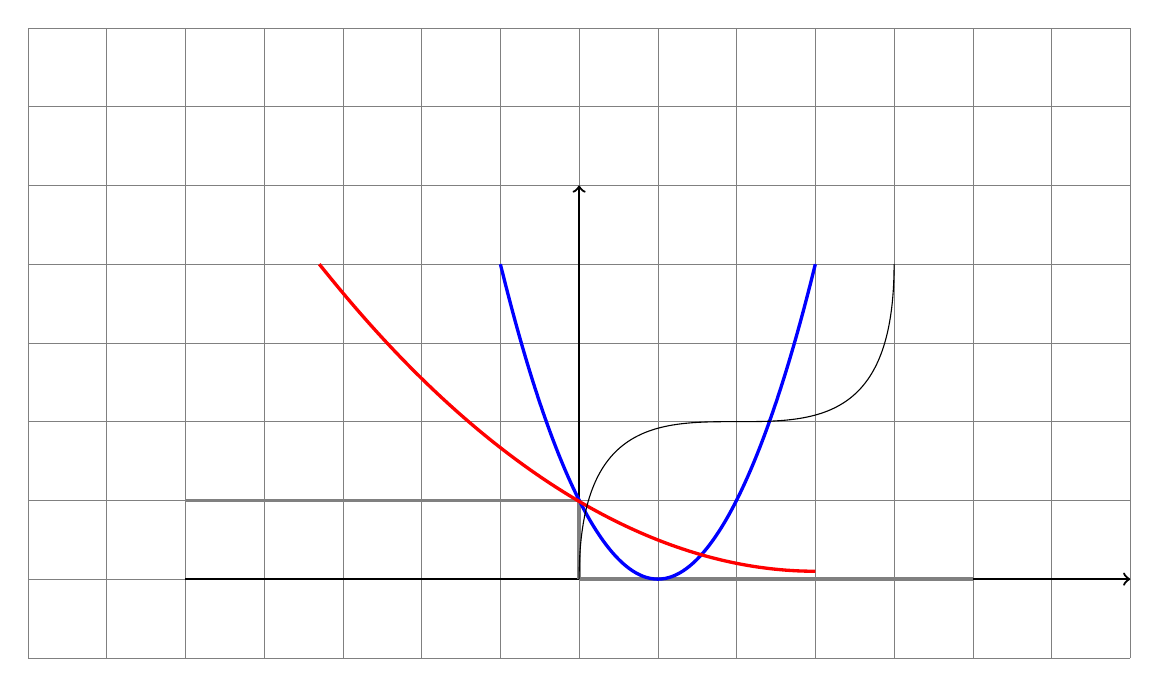
\begin{tikzpicture}		
		\draw[step=1cm,gray,very thin] (-7,-1) grid (7,7);
		\draw[thick, black, ->] (-5,0) -- (7,0);
		\draw[thick, black, ->] (0,0) -- (0,5);
		% Ideal miss-classification error		
		\draw[very thick, gray] (-5,1) -- (0,1);
		\draw[very thick, gray] (0,1) -- (0,0);
		\draw[very thick, gray] (0,0) -- (5,0);
		
		\draw[very thick, blue] (-1,4) parabola bend (1,0) (3,4);
		
		\draw[very thick, red] (3,0.1) parabola (-3.3,4);
		
		\draw (0,0) .. controls (0,4) and (4,0) .. (4,4);
		
	\end{tikzpicture}
	\caption{Different error functions: Ideal Miss-classification Error (gray line)}
\end{figure}

\section{Ideal Miss-classification Error}
Gradient = 0 $\Rightarrow$ can't use gradient descent.\\
It simply counts incorrectly classified points.

\section{Squared Error - $L_2$ Loss}
\begin{itemize}
	\item Leads to closed form solutions
	\item Sensitive to outliers
	\item Penalize "too correct" data points
\end{itemize}

\section{Cross Entropy Error}
\begin{itemize}
	\item Concave function $\Rightarrow$ unique minimum exists
	\item Robust to outliers, error increases only roughly linear
	\item No closed-form solution, requires iterative method
\end{itemize}

\section{Squared Error on Sigmoid / Tanh}
\begin{itemize}
	\item No penalty for "too correct" points
	\item Zero gradient for confidently incorrect classifications
\end{itemize}
$\Rightarrow$ \hlr{Do NOT} use $L_2$ loss with sigmoid outputs, instead, use cross-entropy.

\section{Hinge Error}
\begin{itemize}
	\item Robust to outliers
	\item Zero error for points outside margin $\Rightarrow$ sparsity
	\item Not differentiable around $z_n = 1$
\end{itemize}
\note Want the correct class to have a score that is higher than incorrect class by a fixed margin $\Delta$.
\begin{equation}
	L_i = \sum_{j \neq y_i} \text{max}(0, s_j - s_{y_i} + \Delta)
\end{equation}
in which, $s_j$ is other classes score, $s_{y_i}$ is real class score.

\section{$L_1, L_0$ Loss}
Median, no wrong points

\begin{align}
	&L_1 = \sum |t-y| \\
	&L_2 = \sum (t-y)^2
\end{align}

\section{Average Loss}
Mathematically, dividing the loss by the amount of data $N$ (in each batch or epoch) doesn't have any effect on the result. However, it's usually advisable to take the average to have more meaningful judgment and avoiding overflow when there are numerous data points.
% !TeX spellcheck = en_US
\chapter{Neural Network}

\section{Gradient Descent}
\note Just use ADAM??

\subsection{Vanilla Gradient Descent}
\begin{equation}
	\theta_{t+1} = \theta_t - \eta\nabla_\theta f(\theta_t)
\end{equation}
Check derivative:
\begin{equation}
	f'(x) \approx \frac{f(x+\varepsilon) - f(x-\varepsilon)}{2\varepsilon} \;\;\;\;\; \text{(numerical gradient)}
\end{equation}

\subsection{Momentum}
\begin{itemize}
	\item Init: $v_{dW_0} = 0, v_{db_0} = 0$
	\item Calculate $dW, db$
	\item Update $W, b$
	\begin{equation}
		\Rightarrow \begin{cases}
			v_{dW} &= \beta v_{dW} + (1-\beta)dW\\
			v_{db} &= \beta v_{db} + (1-\beta)db
		\end{cases}
		\Rightarrow
		\begin{cases}
			W &= W - \alpha v_{dW}\\
			b &= b - \alpha v_{db}
		\end{cases}
	\end{equation}
	The above formulas are to calculate the moving average of $v_{dW}$ and $v_{db}$.
	\item Tips: Choose \hlre{\beta_1=0.9}, implying taking average of the last 10 steps.
	\item Reference source: \href{https://youtu.be/k8fTYJPd3_I}{DeepLearning.AI}.
\end{itemize}

\subsection{Nesterov Accelerated Gradient}
\ac{nag}:
\begin{equation}
	v_t = \gamma v_{t-1} + \eta \nabla_tJ\left(\theta - \gamma v_{t-1}\right)
\end{equation}

\subsection{\ac{rmsprop}}
\begin{itemize}
	\item Init $s_{dW_0} = 0, s_{db_0}=0$
	\item Calculate $dW, db$
	\item Update $W, b$
	\begin{equation}
		\begin{cases}
			s_{dW} &= \beta s_{dW} + (1-\beta)dW^2 \\
			s_{db} &= \beta s_{db} + (1-\beta)db^2
		\end{cases}
		\Rightarrow
		\begin{cases}
			W &= W - \alpha \frac{dW}{\sqrt{s_{dW}} + \varepsilon}\\
			b &= b - \alpha \frac{db}{\sqrt{s_{db}} + \varepsilon}
		\end{cases}
	\end{equation}
	\item Tips: choose \hlre{\beta_2 = 0.999, \;\;\varepsilon = 10^{-7}}
	\item Reference source: \href{https://youtu.be/_e-LFe_igno}{DeepLearning.AI}.
\end{itemize}

\subsection{\ac{adam}}
\ac{adam} is basically the combination of Momentum and \ac{rmsprop}.
\begin{itemize}
	\item Init $v_{dW_0}, s_{dW_0}, v_{db_0}, s_{db_0}=0$
	\item Calculate $dW, db$
	\item Update $W, b$
	\begin{equation}
		\begin{cases}
			v_{dW} &= \beta_1 v_{dW} + (1-\beta_1)dW \\
			v_{db} &= \beta_1 v_{db} + (1-\beta_1)db \\
			s_{dW} &= \beta_2 s_{dW} + (1-\beta_2)dW^2 \\
			s_{db} &= \beta_2 s_{db} + (1-\beta_2)db^2
		\end{cases}
		\Rightarrow
		\begin{cases}
			v^{cor.}_{dW} &= \frac{v_{dW}}{1 - \beta_1^t} \\
			v^{cor.}_{db} &= \frac{v_{db}}{1 - \beta_1^t} \\
			s^{cor.}_{dW} &= \frac{s_{dW}}{1 - \beta_2^t} \\
			s^{cor.}_{db} &= \frac{s_{db}}{1 - \beta_2^t}
		\end{cases}
		\Rightarrow
		\begin{cases}
			W &= W - \alpha \frac{v^{cor.}_{dW}}{\sqrt{s^{cor.}_{dW}} + \varepsilon}\\
			b &= b - \alpha \frac{v^{cor.}_{db}}{\sqrt{s^{cor.}_{db}} + \varepsilon}
		\end{cases}
	\end{equation}
	\item Tips: choose \hlre{\beta_1 = 0.9, \;\;\beta_2 = 0.999, \;\;\varepsilon = 10^{-7}}
	\item Reference source: \href{https://youtu.be/JXQT_vxqwIs}{DeepLearning.AI}.
\end{itemize}
% !TeX spellcheck = en_US
\section{Tips and Tricks}

\begin{itemize}
	\item Shuffling
	\item Data Augmentation: reshape, rescale, crops, zooming, change color (color \ac{PCA})
	\item Normalizing the inputs\\
	Convergence is the fastest if
	\begin{itemize}
		\item The mean of each input variable $=0$
		\item Scale $\Rightarrow$ same covariance
	\end{itemize}
	Mean cancellation $\Rightarrow$ \ac{kl} expansion $\Rightarrow$ covariance equalization (if possible)
	\item Leaky \ac{relu} is better a bit than \ac{relu}, ELU
	\item Weights initialization: Xavier-Glorot:
	\[ W \sim U\left(0, \sqrt{\frac{6}{n_{in} + n_{out}}}\right) \]
	\item Batch Norm(alization): Normalize after each layer\\
	$\Rightarrow$ learn the moving average
	\item Drop out\\
	\note When in inferencing (after training), must multiply the activation output with the \ac{prob} that the weights are set to 0
\end{itemize}
\include{Contents/word-embeddings.tex}
% !TeX spellcheck = en_US
\chapter{Search Algorithms}

\hlr{Search problem} is one common type of problem which has numerous presences in our lives. The well-known \ac{TSP} and its variants are search problems, in which the salesman have to find the shortest route that visit every cities. Many \ac{RL} problems can also be viewed as search problems, in which the machine find the most optimal plan to reach the goal.

A search problem consists of: an agent in a state space, a successor function, a start state and a goal state. The \hlr{agent} is the one taking the \hlr{action}, \eg, in \ac{TSP}, the agent is the salesman, and the action is to travel; in \ac{RL}, the agent is the robot or the machine, and the action could be to move to a different position. The \hlr{search state} represents the current situation that the agent is in, which would not necessary equivalent to the world state, which includes every possible details about the environment. \Eg, in \ac{TSP}, the state is the current city, every time the action traveling is taken, the agent moves from one city to another (one state to another). The \hlr{successor function} describes the transition from one state to another. This function usually comes with the transition action and costs.

A \hlr{solution of search problem} is a sequence of actions (a plan) which transform the start state to a goal state. \hlr{Search algorithms} find search solutions, which can be optimal, but in many practical cases, close to optimal within time limitation.

This chapter structures as follows:
\begin{itemize}
	\item The first section describes how a search problem is formulated mathematically as a graph.
	\item The second section presents some well-known search algorithms.
\end{itemize}

\section{Graph}

A graph is the mathematical representation of a search problem. A graph consists of nodes and edges.

\subsection{Undirected Graph}

\subsection{Directed Graph}

\subsection{Adjacency Matrix}

\subsection{Incidence Matrix}

\subsection{Trees and Forest}

\section{Search Algorithms}

\subsection{Properties}

\subsection{Depth-first search}

\subsection{Breadth-first search}

\subsection{Prim's Algorithm}

\subsection{Kruskal's Algorithm}

\subsection{Dijkstra's Algorithm}

\subsection{Bellman and Ford's Algorithm}

\subsection{A* Algorithm}

\todo{}

% !TeX spellcheck = en_US
\chapter{Variational Autoencoders}

\section{Basics Definitions}
\label{sec:vae-defs}
\begin{itemize}
	\item \textit{Probabilistic model}: is a model that represents a probability distribution. It could be a marginal \ac{prob} distribution $p(x)$ or a conditional \ac{prob} distribution $p(y|x)$.
	\item \textit{Evidence, query, and latent variables}:\\
	The word \hlb{latent} implies existing, but hidden. \Eg"
	\begin{itemize}
		\item In $p(x)$, $x$ is the query variable and there is no evidence variable.
		\item In $p(y|x)$, $y$ is the query variable and $x$ is the evidence variable.
		\item In \ac{MoG} $p(x) = \sum_z p(x|z) p(z)$, $x$ is the query variable, $z$ is the latent variable to represent the mixture elements.		
		\item In $p(y|x) = \sum_z p(y|x,z) p(z)$, $z$ is the latent variable.
		\item In a neural network, the inputs are evidence variables, the output are the query variables, and all \ac{param} for the hidden layers can be considered as latent variables, though that would not be a helpful way of consideration. In \ac{VAE}, only $z$ is considered as the latent variable with a simple Gaussian distribution.
		\item In model-based \ac{RL} with latent variable models, $x_t$ is the latent variable.
	\end{itemize}
	\item \textit{Latent variable models}: is the type of probabilistic model that represent a complex \ac{pdf} as the product of multiple simpler \ac{pdf}s, one of which belongs to a latent variable. \Eg: in \ac{VAE}, we has $p(z)$ as an \textit{easy} \ac{pdf} (\eg, Gaussian), $p(x|z)$ as a learnable neural network, then we represent the complex $p(x)$ as:
	\[ p(x) = \int p(x|z) p(z) dz \]
\end{itemize}

\section{Variational Inference}
This section describes how to calculate $p(z|x_i)$

\section{References}
\begin{itemize}
	\item \href{https://www.youtube.com/watch?v=5WoItGTWV54}{Generative models | CS231, Stanford | YouTube}
	\item \href{https://www.youtube.com/watch?v=9zKuYvjFFS8}{Variational Autoencoders | Arxiv Insights | YouTube}
	\item \href{https://www.youtube.com/watch?v=fcvYpzHmhvA}{Variational Autoencoders | CodeEmporium | YouTube}
	\item \href{https://github.com/vdumoulin/conv_arithmetic}{Real "deconv" layer | GitHub}
\end{itemize}
\include{Contents/MDP.tex}
\include{Contents/RL.tex}
% !TeX spellcheck = en_US
\chapter{Probabilistic Robotics}

Reference from the great book: \cite{thrun2006probalistic}.

\section{State Estimation}
\subsection{Bayes Filters}
\begin{align*}
	&bel(x_t) = p(x_t | z_{1:t}, u_{1:t}) && \text{belief over a state}\\
	&\overline{bel}(x_t) = p(x_t | z_{1:t-1}, u_{1:t}) && \text{a posterior (before adapt to }z_t)\\
	\Rightarrow\; & \text{Calculating } bel(x_t) \text{ from  } \overline{bel}(x_t) && \text{correction/measurement update}
\end{align*}

\hlr{\underline{Bayes Filter Algorithm:}}
\begin{align*}
	&2 \qquad \text{for all } x_t \text{ do:}\\
	&3 \qquad \overline{bel}(x_t) = \int p(x_t | u_t, x_{t-1}) bel(x_{t-1}) dx && \text{prediction step}\\
	&4 \qquad bel(x_t) = \eta\, p(z_t | x_t)\, \overline{bel}(x_t) && \text{update step}
\end{align*}\\
$\Rightarrow\;$ Can only be implemented for very simple estimation problems, finite state space

\hlr{\underline{Important assumption:} Markov property} (each state s a complete summary of the past)

\hlr{Problem:} can not be implemented on digital computers

The next subsections describe two Gaussian filters (\ac{KF} and \ac{IF}) and two extensions of them (\ac{EKF} and \ac{EIF}). The Gaussian filters have major advantage in computational cost, with the disadvantage of having assumption on uni-model distribution.

\subsection{The Kalman Filter (KF)}

\begin{itemize}
	\item \hlb{Learning Resources:} \href{http://www.bzarg.com/p/how-a-kalman-filter-works-in-pictures/}{www.bzarg.com}
	\item For continuous space, not discrete or hybrid\\
	\item \hlr{Assumption:} posterior are Gaussians and Markov property\\
	\begin{align*}
		&p(x_t | u_t, x_{t-1}) && \text{must be linear \ac{func} (linear system dynamics)}\\
		&p(z_t, x_t) && \text{also linear}\\
		&bel(x_0) && \text{initial belief must be Gaussian}
	\end{align*}
\end{itemize}

\begin{align*}
	x_t &= A_t x_{t-1} + B_t u_t + \varepsilon_t\\
	p(x_t | u_t, x_{t-1}) &= \det \left( 2\pi\Sigma_t \right)^{-\frac{1}{2}} \exp\left[ -\frac{1}{2} \left( x_t - A_t x_{t-1} - B_t u_t \right)^T R_t^{-1} \left( x_t - A_t x_{t-1} - B_t u_t \right) \right]\\
	z_t &= C_t x_t + \delta_t \quad(=y)\\
	p(z_t | x_t) &= \det \left( 2\pi Q_t \right)^{-\frac{1}{2}} \exp\left[ -\frac{1}{2} \left( z_t - C_t x_t \right)^T Q_t^{-1} \left( z_t - C_t x_t \right) \right]\\
	bel(x_0) = p(x_0) &= \det \left( 2\pi\Sigma_0 \right)^{-\frac{1}{2}} \exp\left[ -\frac{1}{2} \left( x_t - \mu_0 \right)^T \Sigma_0^{-1} \left( x_t - \mu_0 \right) \right]
\end{align*}

\hlr{\underline{Kalman Filter Algorithm:}} $(\mu_{t-1}, \Sigma_{t-1}, u_t, z_t)$
\begin{align*}
	&\begin{rcases}
		2 \qquad \overline{\mu}_t = A_t \mu_{t-1} + B_t u_t\\
		3 \qquad \overline{\Sigma}_t = A_t \Sigma_{t-1} A_t^T + R_t \qquad\qquad\qquad\qquad\qquad\quad
	\end{rcases} \text{incorporate } u_t \text{ - prediction step - } \mathcal{O}(n^2)\\
	&\begin{rcases}
		4 \qquad K_t = \overline{\Sigma}_t C_t^T \left( C_t \overline{\Sigma}_t C_t^T + Q_t \right)^{-1} \qquad \text{(Kalman gain)}\\
		5 \qquad \mu_t = \overline{\mu}_t + K_t (z_t - C_t \overline{\mu}_t)\\
		6 \qquad \Sigma_t = (I - K_t C_t) \overline{\Sigma}_t
	\end{rcases} \text{incorporate } z_t \text{ - correction step - } \mathcal{O}(n^{2,8})\\
	&\;7 \qquad  \text{return } \mu_t, \Sigma_t \qquad\qquad\qquad\qquad\qquad\quad\qquad\qquad\Rightarrow\; \text{belief at time } t
\end{align*}
$\Rightarrow$ quite computationally expensive, \hlr{everything are Gaussians}

\subsection{Extended Kalman Filter (EKF)}
Overcome the assumption on linearity by only approximate by Gaussians
\begin{align*}
	x_t &= g(u_t, x_{t-1}) + \varepsilon_t\\
	z_t &= h(x_t) + \delta_t
\end{align*}

\begin{align*}
	g(u_t, x_{t-1}) &\approx g(u_t, \mu_{t-1}) + g'(u_t, \mu_{t-1}) (x_t - \mu_{t-1}) \\
	&= g(u_t, \mu_{t-1}) + G_t(x_t - \mu_{t-1})\\
	& g' \text{ is the Jacobian of state } (n\times n \text{ matrix})\\
	p(x_t | u_t, x_{t-1}) &\approx \det \left( 2\pi R_t \right)^{-\frac{1}{2}} \exp \left\{-\frac{1}{2} [x_t - g(u_t, x_{t-1})] ^T R_t^{-1} [x_t - g(u_t, x_{t-1})] \right\} \\
	h(t) &\approx h(\overline{\mu}_t) + h'(\mu_t) (x_t - \mu_{t-1})\\
	&= h(\overline{\mu}_t) + H_t (x_t - \mu_{t-1})\\
	p(z_t | x_t) &= \det \left( 2\pi Q_t \right)^{-\frac{1}{2}} \exp \left\{-\frac{1}{2} [z_t - h(x_t)] ^T Q_t^{-1} [z_t - h(x_t)]\right\} \\
\end{align*}

\hlr{\underline{Extended Kalman Filter Algorithm:}} $(\mu_{t-1}, \Sigma_{t-1}, u_t, z_t)$
\begin{align*}
	&2 \qquad \overline{\mu}_t = g(u_t, \mu_{t-1})\\
	&3 \qquad \overline{\Sigma}_t = G_t \Sigma_{t-1} G_t^T + R_t\\
	&4 \qquad K_t = \overline{\Sigma}_t H_t^T \left( H_t \overline{\Sigma}_t H_t^T + Q_t \right)^{-1} \\
	&5 \qquad \mu_t = \overline{\mu}_t + K_t [z_t - h(\overline{\mu}_t)]\\
	&6 \qquad \Sigma_t = (I - K_t H_t) \overline{\Sigma}_t\\
	&7 \qquad \text{return } \mu_t, \Sigma_t
\end{align*}

\begin{itemize}
	\item Can extend \ac{EKF} $\Rightarrow$ \ac{MHEKF}
	\item \ac{EKF}'s performance depends on degree of nonlinearities and uncertainty
	\item Unscented \ac{KF} and moments matching \ac{KF} are better
\end{itemize}

\subsection{Information Filter (IF)}
\begin{itemize}
	\item Moment representation:\tab\tab $\mu \quad\&\quad \Sigma$
	\item Canonical representation:\tab\tab $\xi \quad\&\quad \Omega$\\
	Information \ precision matrix: \tab $\Omega = \Sigma^{-1};\qquad \Sigma = \Omega^{-1}$\\
	Information vector: \tab \tab \tab $\xi = \Sigma^{-1}\mu;\qquad \mu = \Omega^{-1}\xi$
\end{itemize}
\begin{align*}
	p(x) &= \det(2\pi\Sigma)^{-\frac{1}{2}} \exp \left\{-\frac{1}{2} (x-\mu)^T \Sigma^{-1} (x-\mu) \right\}\\
	&= \eta \exp\left\{ -\frac{1}{2} x^T\Omega x + x^T \xi \right\}
\end{align*}

\hlr{\underline{Information Filter Algorithm:}} $(\xi_{t-1}, \Omega_{t-1}, u_t, z_t)$
\begin{align*}
	&\begin{rcases}
		2 \qquad \overline{\Omega}_t = (A_t \Omega_{t-1}^{-1} A_t^T + R_t)^{-1} \qquad\qquad\\
		3 \qquad \overline{\xi}_t = \overline{\Omega}_t ( A_t \Omega_{t-1}^{-1} \xi_{t-1} + B_t u_t )
	\end{rcases} \mathcal{O}(n^{2,8})\\
	&\begin{rcases}
		4 \qquad \Omega_t = C_t^T Q_t^{-1} C_t + \overline{\Omega}_t\\
		5 \qquad \xi_t = C_t^T Q_t^{-1} z_t + \overline{\xi}_t \qquad\qquad\qquad\quad
	\end{rcases} \mathcal{O}(n^2)\\
	&\;6 \qquad \text{return } \xi_t, \Omega_t
\end{align*}

\subsection{Extended Information Filter (IF)}
\begin{align*}
	x_t &= g(u_t, x_{t-1}) + \varepsilon_t\\
	z_t &= h(x_t) + \delta_t\\
	G_t &= g'(u_t, \mu_{t-1})\\
	H_t &= h'(\mu_t)
\end{align*}

\hlr{\underline{Extended Information Filter Algorithm:}} $(\xi_{t-1}, \Omega_{t-1}, u_t, z_t)$
\begin{align*}
	&2 \qquad \mu_{t-1} = \Omega_{t-1}^{-1} \xi_{t-1}\\
	&3 \qquad \overline{\Omega}_t = (G_t \Omega_{t-1}^{-1} G_t^T + R_t)^{-1}\\
	&4 \qquad \overline{\xi}_t = \overline{\Omega}_t\, g(u_t, \mu_{t-1})\\
	&5 \qquad \overline{\mu}_t = g(u_t, \mu_{t-1})\\
	&6 \qquad \Omega_t = \overline{\Omega}_t + H_t^T Q_t^{-1} H_t\\
	&7 \qquad \xi_t = \overline{\xi}_t + H_t^T Q_t^{-1} \left[ z_t - h(\overline{\mu}_t) - H_t \overline{\mu}_t \right]
\end{align*}

\begin{itemize}
	\item \hlb{Global uncertainty:} set $\Omega=0$ is better than set $|\Sigma| = \infty$
	\item \ac{IF} tends to be numerically more stable than \ac{KF}
	\item \ac{IF} is better for multi-robot problems
	\item For high dimensional state, \ac{EKF} is computational better than \ac{EIF}
\end{itemize}

\section{Measurements}
\subsection{Map Representation}
Maps: $m = \{ m_1, m_2, \dots, m_N \}$\\
\hlr{There are \underline{2 ways} to represent a map:}
\begin{table}[hbt!]
	\centering
	\begin{tabular}{c|c}
		feature-based & location-based \\\hline\hline
		$m_n$: properties of a feature and location of feature & a specific location \\\hline
		\hlr{only the shape} of the environment & volumetric: \hlr{label for any location} \\
		\hlr{at the specific locations} & in the world\\\hline
		easy to adjust positions of objects & occupancy grid map \\
		$\Rightarrow$ popular in the robotic mapping field &
	\end{tabular}
\end{table}

\todo{Add images}

\subsection{Measurement Noise}
The 4 types of measurement noise:
\begin{itemize}
	\item Correct range with local measurement noise\\
	With $z_t^{k*}$ as the correct distance
	\begin{equation}
		p_{hit}(z_t^k | x_t, m) = \begin{cases}
			\eta\; \mathcal{N}(z_t^k| z_t^{k*}, \sigma^2_{hit}) \qquad \text{if } 0 \leq z_t^k \leq z_{\max}\\
			0 \qquad\qquad\qquad\qquad\quad \text{otherwise}
		\end{cases}
	\end{equation}
	\item Unexpected object
	\begin{equation}
		p_{short}(z_t^k | x_t, m) = \begin{cases}
			\eta\lambda_{short} e^{-\lambda_{short} z_t^k} \qquad \text{if } 0 \leq z_t^k \leq z_t^{k*}\\
			0 \qquad\qquad\qquad\qquad \text{otherwise}
		\end{cases}
	\end{equation}
	\item Failures
	\begin{equation}
		p_{\max}(z_t^k | x_t, m) = I(z=z_{\max})
	\end{equation}
	\item Random measurements
	\begin{equation}
		p_{rand}(z_t^k | x_t, m) = \begin{cases}
			\frac{1}{z_{\max}} \qquad \text{if } 0 \leq z_t^k < z_{\max}\\
			0 \qquad\quad \text{otherwise}
		\end{cases}
	\end{equation}
\end{itemize}

\todo{Add image, plot}

\begin{equation}
	p(z_t^k | x_t, m) = \begin{bmatrix}
		z_{hit}\\ z_{short}\\
		z_{max}\\ z_{rand}
	\end{bmatrix}^T . \begin{bmatrix}
		p_{hit}(z_t^k | x_t, m)\\ p_{short}(z_t^k | x_t, m)\\
		p_{max}(z_t^k | x_t, m)\\ p_{rand}(z_t^k | x_t, m)
	\end{bmatrix}
\end{equation}

\section{Robot Motion}
Pose: $[x, y, \theta]^T$ at location $[x, y]^T$ and orientation $\theta$

\subsection{Motion Model}

Motion Model, \ac{aka} Probabilistic Kinematic Model: $p(x_t,  u_t, x_{t-1})$

\begin{table}[hbt!]
	\centering
	\begin{tabular}{c|c}
		Velocity commands & Odometry \\
		& (distance traveled, angle turned, \etc)\\\hline\hline
		& \hlr{more accurate}\\
		& \hlr{but post-the-fact}\\
		& \hlr{(not for motion planning)}\\
		Use for Probabilistic motion planning & Use for estimation
	\end{tabular}
\end{table}

Each has closed form calculation and sampling algorithm.

\subsection{Velocity Motion Model}
Assuming we can control a robot through velocities:
\begin{equation*}
	u_t = \begin{bmatrix}
		v_t\\ \omega_t
	\end{bmatrix}; \qquad
	x_{t-1} = \begin{bmatrix}
		x \\ y \\ \theta
	\end{bmatrix}; \qquad
	x_t = \begin{bmatrix}
		x'\\ y'\\ \theta'
	\end{bmatrix}
\end{equation*}

\hlr{\underline{Motion Model Velocity Algorithm:}} $(x_t, u_t, x_{t-1})$
\begin{align*}
	& \begin{rcases} \displaystyle
		2 \qquad \mu = \frac{1}{2} \frac{(x-x')\cos\theta+(y-y')\sin\theta}{(y-y')\cos\theta-(x-x')\sin\theta} \qquad\qquad\\
		3 \qquad x^* = \frac{x+x'}{2} + \mu (y-y')\\
		4 \qquad y^* = \frac{y+y'}{2} + \mu (x'-x)\\
		5 \qquad r^* = \sqrt{(x-x^*)^2 + (y-y^*)^2}
	\end{rcases} \text{Invert the motion model}\\
	& \;6 \qquad \Delta \theta = \text{atan2}(y'-y^*, x'-x^*) - \text{atan2}(y-y^*, x-x^*)\\
	& \begin{rcases}
		7 \qquad\hat{v} = \frac{\Delta\theta}{\Delta t} r^*\\
		8 \qquad\hat{\omega} = \frac{\Delta\theta}{\Delta t}\\
		9 \qquad\hat{\gamma} = \frac{\theta' - \theta}{\Delta t} - \hat{\omega}
		\qquad\qquad
	\end{rcases} \text{compared actual velocities with the desired}\\
	& 10 \qquad \text{return } p(v-\hat{v}, \alpha_1|v| + \alpha_2|\omega|) 
	\cdot p(\omega-\hat{\omega}, \alpha_3|v| + \alpha_4|\omega|)
	\cdot p(\hat{\gamma}, \alpha_5|v| + \alpha_6|\omega|)
\end{align*}

\hlr{\underline{Sample Motion Model Velocity Algorithm:}} $(u_t, x_{t-1})$
\begin{align*}
	& 2 \qquad \hat{v} = v + sample(\alpha_1|v| + \alpha_2|\omega|) \\
	& 3 \qquad \hat{\omega} = \omega + sample(\alpha_3|v| + \alpha_4|\omega|) \\
	& 4 \qquad \hat{\gamma} = sample(\alpha_5|v| + \alpha_6|\omega|) \\
	& 5 \qquad x' = x - \frac{\hat{v}}{\hat{\omega}}\sin\theta + \frac{\hat{v}}{\hat{\omega}}\sin(\theta + \hat{\omega}\Delta t)\\
	& 6 \qquad y' = y + \frac{\hat{v}}{\hat{\omega}}\cos\theta - \frac{\hat{v}}{\hat{\omega}}\cos(\theta + \hat{\omega}\Delta t)\\
	& 7 \qquad \theta' = \theta + \hat{\omega} \Delta t + \hat{\gamma} \Delta t \\
	& 8 \qquad \text{return } x_t = [x', y', \theta']^T
\end{align*}

\begin{itemize}
	\item Probability normal distribution(a, b): \qquad return $\displaystyle \frac{1}{\sqrt{2\pi b}}e^{-\frac{a^2}{2b}}$
	\item Probability triangular distribution(a, b): \qquad return $\displaystyle \begin{cases}
		0 \qquad\qquad \text{if } |a| > \sqrt{6b}\\
		\frac{\sqrt{6b} - |a|}{6b} \qquad \text{else}
	\end{cases}$
	\item Sample normal distribution(b): \qquad return $\displaystyle \frac{b}{6} \sum_{i=1}^{12} rand(-1, 1)$
	\item Sample triangle distribution(b): \qquad return $b.rand(-1,1).rand(-1,1)$
\end{itemize}

\subsection{Odometry Motion Model}
Only available after the robot has moved\\
$\Rightarrow$ only use for filter algorithm\\
not for accurate motion planning and control

\hlr{\underline{Motion Model Odometry Algorithm:}} $(x_t, u_t, x_{t-1})$
\begin{align*}
	& \;2 \qquad \delta_{rot1} = \text{atan2}(\bar{y}'-\bar{y}, \bar{x}'-\bar{x}) - \bar{\theta} \\
	& \;3 \qquad \delta_{trans} = \sqrt{(\bar{x}-\bar{x}')^2 + (\bar{y}-\bar{y}')^2} \\
	& \;4 \qquad \delta_{rot2} = \bar{\theta}' - \bar{\theta} - \delta_{rot1} \\
	& {\color{red} \begin{rcases}
		{\color{black} 5 \qquad \hat{\delta}_{rot1} = \text{atan2}(y'-y, x'-x) - \theta} \qquad\qquad \\
		{\color{black} 6 \qquad \hat{\delta}_{trans} = \sqrt{(x-x')^2 + (y-y')^2}} \\
		{\color{black} 7 \qquad \hat{\delta}_{rot2} = \theta' - \theta - \hat{\delta}_{rot1}}
	\end{rcases} \Rightarrow \text{inverse motion model}} \\	
	& \;8 \qquad p_1 = prob(\delta_{rot1} - \hat{\delta}_{rot1}, \alpha_1 \hat{\delta}_{rot1} + \alpha_2 \hat{\delta}_{trans}) \\
	& \;9 \qquad  p_2 = prob(\delta_{trans} - \hat{\delta}_{trans}, \alpha_3 \hat{\delta}_{trans} + \alpha_4 (\hat{\delta}_{rot1} + \hat{\delta}_{rot2})) \\
	& 10 \qquad  p_3 = prob(\delta_{rot2} - \hat{\delta}_{rot2}, \alpha_1 \hat{\delta}_{rot2} + \alpha_2 \hat{\delta}_{trans}) \\
	& 11 \qquad \text{return}\quad p_1.p_2.p_3 \qquad (=p(x_t| u_t, x_{t-1}))
\end{align*}

\note
\begin{itemize}
	\item Bar $\Leftrightarrow$ measurements
	\begin{align*}
		\overline{x}_{t-1} &= [\bar{x} \quad \bar{y} \quad \bar{\theta}]^T\\
		\overline{x}_t &= [\bar{x}' \quad \bar{y}' \quad \bar{\theta}']^T
	\end{align*}
	\item Hat $\Leftrightarrow$ estimations
	\item No bar and hat $\Leftrightarrow$ hypothesized final pose $x, y$
\end{itemize}

\hlr{\underline{Sample Motion Model Odometry Algorithm:}} $(u_t, x_{t-1})$
\begin{align*}
	2 \qquad & \delta_{rot1} = \text{atan2}(\bar{y}'-\bar{y}, \bar{x}'-\bar{x}) - \bar{\theta} \\
	3 \qquad & \delta_{trans} = \sqrt{(\bar{x}-\bar{x}')^2 + (\bar{y}-\bar{y}')^2} \\
	4 \qquad & \delta_{rot2} = \bar{\theta}' - \bar{\theta} - \delta_{rot1} \\
	5 \qquad & \hat{\delta}_{rot1} = \delta_{rot1} - sample(\alpha_1\delta_{rot1} + \alpha_2\delta_{trans}) \\
	6 \qquad & \hat{\delta}_{trans} =\delta_{trans} - sample(\alpha_3\delta_{trans} + \alpha_4(\delta_{rot1} + \delta_{rot2}) )\\
	7 \qquad & \hat{\delta}_{rot2} = \delta_{rot2} - sample(\alpha_1\delta_{rot2} + \alpha_2\delta_{trans}) \\
	8 \qquad & x' = x + \hat{\delta}_{trans} \cos(\theta + \hat{\delta}_{rot1})\\
	9 \qquad  & y' = y + \hat{\delta}_{trans} \sin(\theta + \hat{\delta}_{rot1})\\
	10 \qquad  & \theta' = \theta + \hat{\delta}_{rot1} + \hat{\delta}_{rot2} \\
	11 \qquad & \text{return}\quad x_t = [x' \quad y' \quad \theta']^T
\end{align*}

\subsection{Map-based Motion Model}

Map-based Motion Model: $p(x_t | u_t, x_{t-1}, m)$
\begin{itemize}
	\item Occupancy maps: $p(x_t | m) = 0 \Leftrightarrow$ the robot collides
	\item If the distance from $x_{t-1} \rightarrow x_t$ is small enough (< half the robot's diameter), we can estimate the \ac{prob} $p(x_t | u_t, x_{t-1}, m) \approx \eta p(x_t | u_t, x_{t-1})p(x_t | m)$, which discards the info relating the robot's path to $x_t$
\end{itemize}

\hlr{\underline{Motion Model with Map Algorithm:}} $(x_t, u_t, x_{t-1}, m)$\\
return $p(x_t | u_t, x_{t-1}).p(x_t | m)$

\hlr{\underline{Sample Motion Model with Map Algorithm:}} $(u_t, x_{t-1}, m)$\\
\begin{align*}
	&do:\\
	& \qquad x_t = sample\_motion\_model(u_t, x_{t-1})\\
	& \qquad \pi = p(x_t | m)\\
	&until \quad \pi > 0\\
	&return <x_t, \pi>
\end{align*}

\backmatter
\pagenumbering{Roman}
\printbibliography[heading=bibintoc]
\appendix
\end{document}